\documentclass[10pt,a4paper]{article}

\usepackage[T1]{fontenc}
\usepackage[utf8]{inputenc}
\usepackage{ae}
\usepackage{aecompl}
\usepackage{zefonts}
\usepackage{multicol}
\usepackage{array, multirow, tabularx}
\usepackage{makecell}
\usepackage{graphicx}
% \usepackage{picins}
\usepackage{amsfonts,amsmath,amssymb}
\usepackage{eurosym}
\usepackage{ulem} %permet de barrer sdu texte avec \sout{} , hachurer avec \xout , souligner avec vaguelette \uwave
\usepackage{textcomp}
\usepackage{graphicx}
\usepackage{yhmath} %arc de cercle avec $\wideparen{AB}$
\usepackage[np]{numprint} %espacement grands nombres
\usepackage{fdsymbol} % symbole calculatrice casio
\usepackage{enumerate}
\usepackage{fancybox} % shadowbox etc...
\usepackage{pifont}
\usepackage{tabularx} 
\usepackage{boxedminipage}
\usepackage[thmmarks,framed]{ntheorem}   %fonction  \newtheorem améliorée incompatible avec amsthm
\usepackage{framed}
\usepackage{titlesec}
\usepackage{colortbl} %charge xcolor , à mettre avant tikz sinon conflit...
\usepackage{pgfkeys} % repères avec tikz
\usepackage{tikz}
\usepackage{tkz-tab} %tableaux de variation
\usepackage{esvect} %vecteurs
\usepackage{pgf} %exporter figures geogebra
\usepackage{mathrsfs} %exporter figures geogebra
\usepackage{slashbox} %sépare une cellule en 2 dans un tableau \backslashbox{Texte dessous}{Texte dessus}
\usepackage{diagbox} %\diagbox{}{}
\usetikzlibrary{arrows} %exporter figures geogebra
\usepackage[french,frenchkw,algoruled]{algorithm2e} %algo 
%\usepackage{algorithm} %algo style algobox
% \usepackage{algpseudocode}% algo style algobox
% \input algtolatex %algo style algobox - nécessite le fichier algolatex.
\usepackage{calrsfs} % plus belles majuscules avec \mathcal
% \usepackage{sesamanuel} % pour les commandes spéciales du manuel 2de
% \usepackage{sesamanuelTIKZ} % pour les commandes spéciales de la figure
%\usepackage{stmaryrd} %double crochet avec \llbracket et rrbracket$
\usepackage{qrcode} %qrcode cliquable \qrcode[height=taille]{adresse}
\usepackage{hyperref} %lien hypertexte \href{adresse}{texte}
%\usepackage[xcas]{pro-graphes} %graphe and co
%\usepackage{dijkstra}
\usepackage{tcolorbox} %cadres plus jolis
\usepackage{karnaugh-map} %permet de tracer des tableaux de Karnaugh
%\usepackage{graphicx}
\usepackage[export]{adjustbox} % Alignement vertical images avec b,t,c \includegraphics[scale=1,valign=t]{Image.png}
\usepackage{fancyvrb} % verbatim amélioré \begin{Verbatim}[frame=single,label=,numbers=left] etc [frame=single/leftline/topline/bottomline/lines] framerule=1mm framesep=5mm rulecolor=\color{red} fillcolor=\color{yellow}
\usepackage[load-configurations = abbreviations]{siunitx}
%\sisetup{locale = FR,detect-all,inter-unit-product= \cdot} %norme SI pour les nombres et unités 
%\SI{25000}{mm} \SI{6.022e23}{\per\mol}  \SI{300}{\watt\per\square\meter} \SI{300}{W / m^2} \SI[per-mode=symbol]{210}{\km\per\hour}
% unité seule \si{\newton\meter} nombre seul \num{24415.15625}

\usepackage{witharrows} %permet de mattre des flèches entre lignes d'équations \begin{WithArrows}@ \Arrow{@}\\@\end{WithArrows}

\usepackage{xlop} % pose les oprétaions "à la main" \opadd{@}{@}; opsub ; opmul ; opdiv (eucl) ; opidiv
%\usepackage{minted}{Python} % permet d'écrire en Python avec \begin{minted}{Python}@\end{minted}
\usepackage{stmaryrd} % crochets intervalles entiers \llbracket ; \rrbracket ; parall \sslash ; contradiction \lightning

\usepackage{mathtools}

%%%%%%%Compteurs%%%%%%%%%%%%%%%%%%%%%%%%%%%%%%%%%%%%%%%%%%%%%%%%%%%%%%%%%%%%%%%%%%%%%
% \newcounter{defcompt}   %Défintion d'un compteur
% \newcounter{exocompt}
% \newcounter{theocompt}
% \newcounter{propcompt}
% \newcounter{regcompt}
\newcounter{numexos}

\setcounter{numexos}{0} %initialisation du compteur





% Nouvelles commandes
\definecolor{cqcqcq}{rgb}{0.7529411764705882,0.7529411764705882,0.7529411764705882} %gris geogebra

\newcommand{\paral}{~\mathbin{\!/\mkern-5mu/\!}~} % symbole parallèle

\newcommand{\R}{\mathbb{R}}
\newcommand{\N}{\mathbb{N}}
\newcommand{\D}{\mathbb{D}}
\newcommand{\Z}{\mathbb{Z}}
\newcommand{\Q}{\mathbb{Q}}
\newcommand{\C}{\mathbb{C}}
\newcommand{\U}{\mathbb{U}}

\newcommand{\rel}{\mathcal{R}} % relation binaire

\newcommand{\e}{\text{e}} % exponentielle en lettre droite dans $$ 

\newcolumntype{R}[1]{>{\raggedleft\arraybackslash }b{#1}}
\newcolumntype{L}[1]{>{\raggedright\arraybackslash }b{#1}}
\newcolumntype{C}[1]{>{\centering\arraybackslash }b{#1}}

\newcolumntype{G}[1]{>{\raggedright\arraybackslash }X{#1}}
\newcolumntype{D}[1]{>{\raggedleft\arraybackslash }X{#1}}
\newcolumntype{M}[1]{>{\centering\arraybackslash }X{#1}}


\newcommand{\exe}{\textbf{Exemple : }}
\newcommand{\exes}{\textbf{Exemples : }}
\newcommand{\rema}{\textbf{Remarque : }}
\newcommand{\rems}{\textbf{Remarques : }}
\newcommand{\rap}{\textbf{Rappel : }}
\newcommand{\raps}{\textbf{Rappels : }}
\newcommand{\dem}{\textbf{Démonstration : }}
\newcommand{\dems}{\textbf{Démonstrations : }}
\newcommand{\csq}{\textbf{Conséquence : }}







\newcommand{\Ex}[1]{{\sc{Exercice #1:}}}
\newcommand{\defi}[1]{\begin{leftbar}
\textbf{Définition :} {#1}
 \end{leftbar}}
\newcommand{\defis}[1]{\begin{leftbar}
\textbf{Définitions :} {#1}
 \end{leftbar}}
 
\newcommand{\prop}[1]{\begin{framed}
\textbf{Propriété :} {#1}
 \end{framed}} 
 
\newcommand{\props}[1]{\begin{framed}
\textbf{Propriétés :} {#1}
 \end{framed}} 
 
\newcommand{\theo}[1]{\begin{framed}
\textbf{Théorème :} {#1}
 \end{framed}} 
\newcommand{\theos}[1]{\begin{framed}
\textbf{Théorèmes :} {#1}
 \end{framed}}  
 
\newcommand{\reg}[1]{\begin{framed}
\textbf{Règle :} {#1}
 \end{framed}} 
\newcommand{\regs}[1]{\begin{framed}
\textbf{Règles :} {#1}
 \end{framed}}  
 
\newcommand{\propdef}[1]{\begin{framed}
\textbf{Propriété - Définition :} {#1}
 \end{framed}} 
\newcommand{\propsdef}[1]{\begin{framed}
\textbf{Propriétés - Définition :} {#1}
 \end{framed}}  
 
 
 \newcommand{\csqs}[1]{\begin{framed}
 \textbf{Conséquences :} {#1}
 \end{framed}} 
 
\newcommand{\cor}[1]{\begin{framed}
\textbf{Corollaire :} {#1}
 \end{framed}}     
     
     
%\newcommand{\cadre}[2]{
%\begin{tcolorbox}[colback=red!5!white,
%                  colframe=red!75!black,
%                  title={#1}]
%{#2}
%\end{tcolorbox}  }

\newcommand{\cadre}[3]{
\begin{tcolorbox}[colback=#1!5!white,
                  colframe=#1!75!black,
                  title={#2}]
{#3}
\end{tcolorbox}  }




\newcommand*{\Coord}[3]{% 
\ensuremath{\vv{#1}\, 
    \begin{pmatrix} 
      #2\\ 
      #3 
    \end{pmatrix}}} % coordonnées de vecteurs.
    
\newcommand{\fonction}[5]{\begin{tabular}[t]{cccc}
$#1 :$ & $#2$ & $\longrightarrow$ & $#3$ \\
 & $#4$ & $\longmapsto$ & $#5$
\end{tabular}}
    
\newcommand{\att}{{\fontencoding{U}\fontfamily{futs}\selectfont\char 66\relax \quad}}    % symbole attention

\newcommand{\exo}{%Création d'une macro ayant un paramètre
\addtocounter{numexos}{1}%chaque fois que cette macro est appelée, elle ajoute 1 au compteur numexos
{\sc{Exercice\,\thenumexos\,:}}\,%la valeur du compteur appelée par \thenumeexos
}

\newcommand{\bint}{\displaystyle \int\limits} %signe intégral plus grand

\newcommand{\bsum}{\displaystyle \sum} %signe somme plus grand

\newcommand{\bprod}{\displaystyle \prod\limits} %signe produit plus grand

\newcommand*{\norme}[1]{\left\lVert\vv{#1}\right\rVert}  %norme de vecteur

\newcommand{\ps}[2]{\ensuremath{\vv{#1}.\vv{#2}}} %produit scalaire

\newcommand{\x}{\times} %produit

\newcommand{\modulo}{\text{ modulo }} 

\renewcommand{\Im}[1]{\text{Im} (#1)}

\renewcommand{\Re}[1]{\text{Re} (#1)}

\newcommand{\modu}[3]{{#1} \equiv {#2} ~ [{#3}]}


\newcommand*{\sep}[1]{
\dotfill
\vspace*{-0.3cm}
\begin{center}
\textbf{#1}
\end{center}
\vspace*{-0.5cm}
\dotfill}


%Flèches avec commentaire : exemple $\xRightarrow[test1]{test1}$
%\makeatletter
%\newcommand{\xRightarrow}[2][]{\ext@arrow 0359\Rightarrowfill@{#1}{#2}}
%\makeatother
%
%\makeatletter
%\newcommand{\xLeftarrow}[2][]{\ext@arrow 0359\Leftarrowfill@{#1}{#2}}
%\makeatother
%
%\makeatletter
%\newcommand{\xLeftrightarrow}[2][]{\ext@arrow 0359\Leftrightarrowfill@{#1}{#2}}
%\makeatother


% Renouvellement commandes

\renewcommand{\leq}{\leqslant}
\renewcommand{\geq}{\geqslant}
\renewcommand{\thesection}{\Roman{section} )  \hspace{-4mm}}
\renewcommand{\thesubsection}{\quad \arabic{subsection}\hspace{-0.9mm} ) \hspace{-5mm}}
\renewcommand{\thesubsubsection}{\qquad \alph{subsubsection}\hspace{0.5mm} ) \hspace{-5mm}}


% Présentation générale

\newcommand{\titre}[1]{\begin{center} \Large \sc \fbox{{#1}}\end{center}}

\newcommand{\entete}[1]{\begin{center} \large \underline{#1} \end{center}}

\titleformat*{\section}{\large\bfseries}
\titleformat*{\subsection}{\large\bfseries}
\titleformat*{\subsubsection}{\large\bfseries}
\titleformat*{\paragraph}{\large\bfseries}
\titleformat*{\subparagraph}{\large\bfseries}

%\newcommand{\DS}[3]{\begin{tabular}{|L{6cm}|C{5cm}|C{6cm}|}
%\hline 
%Nom : & Devoir Surveillé #1 & Classe \quad :\quad #2 \\ 
%Prénom : &  & #3 \\ 
%\hline 
%\end{tabular} }

\newcommand{\DS}[3]{\begin{tabularx}{1 \linewidth}{|G|M|M|}
\hline 
Nom : & Devoir Surveillé #1 & Classe \quad :\quad #2 \\ 
Prénom : &  & #3 \\ 
\hline 
\end{tabularx} }

\newcommand{\DSBTS}[4]{\begin{tabularx}{1 \linewidth}{|G|M|M|}
\hline 
Nom : & Devoir Surveillé #2 & Classe \quad :\quad #3 \\ 
Prénom : & #1 & #4 \\ 
\hline 
\end{tabularx} }

\newcommand{\DM}[3]{\begin{tabular}{|L{6.1cm}|C{5.6cm}|C{6.1cm}|}
\hline 
Nom : & Devoir à la maison~ #1 & Classe \quad :\quad #2 \\ 
Prénom : &  & Pour le #3 \\ 
\hline 
\end{tabular} }

\newcommand{\ct}[3]{\begin{tabular}{|L{6.1cm}|C{5.6cm}|C{6.1cm}|}
\hline 
Nom : & Contrôle~ #1 & Classe \quad :\quad #2 \\ 
Prénom : &  & #3 \\ 
\hline 
\end{tabular} }

% Repères automatisés avec Tikz 
% Définition des nouvelles options xmin, xmax, ymin, ymax
% Valeurs par défaut : -3, 3, -3, 3
\tikzset{
xmin/.store in=\xmin, xmin/.default=-3, xmin=-3,
xmax/.store in=\xmax, xmax/.default=3, xmax=3,
ymin/.store in=\ymin, ymin/.default=-3, ymin=-3,
ymax/.store in=\ymax, ymax/.default=3, ymax=3,
}
% Commande qui trace la grille entre (xmin,ymin) et (xmax,ymax)
\newcommand {\grille}
{\draw[help lines] (\xmin,\ymin) grid (\xmax,\ymax);}
% Commande \axes
\newcommand {\axes} {
\draw[->] (\xmin,0) -- (\xmax,0);
\draw[->] (0,\ymin) -- (0,\ymax);
}
% Commande qui limite l’affichage à (xmin,ymin) et (xmax,ymax)
\newcommand {\fenetre}
{\clip (\xmin,\ymin) rectangle (\xmax,\ymax);}

% Exemple 
%\begin{center}
%\begin{tikzpicture} [xmin=@,xmax=@,ymin=@,ymax=@]
%\grille \axes \fenetre
%\draw plot[smooth] (\x,@);
%\end{tikzpicture}
%\end{center}

%%%%%%%\newtheorem{}{×}%%%%%%%%%%%%%%%%%%%%%%%%%%%%%%%%%%%%%%%%%%%%%%%%%%%%%%%%%%%%%
%\theoremseparator{\hspace{0.8mm} :}
%{\theoremseparator{~:}
%\newtheorem*{rem}{Remarque}
%\newtheorem*{rems}{Remarques}
%\newframedtheorem{theo}[theocompt]{Théorème}
%\newtheorem{prop}[propcompt]{Propriété}
%\newtheorem{regle}[regcompt]{Règle}
%\newtheorem{defi}[defcompt]{Définition}
%\newtheorem*{voc}{Vocabulaire}}


%algo
%VARIABLES : 
%\Variables
%Début et fin de bloc :
%\DebutAlgo 
%\FinAlgo 
%\DebutPour
%\FinPour
%\DebutTantQue
%\FinTantQue
%\DebutSi
%\FinSi
%\DebutSinon
%\FinSinon
%SI...ALORS :
%\Si{(...)}
%SINON :
%\Sinon
%POUR ... ALLANT_DE ... A ...
%\Pour{...}{...}{...}
%TANT_QUE(...)
%\Tantque{(...)}
%Pour toutes les autres instructions (y compris les déclarations de variable)
%\Ligne ...


% Mise en page
\usepackage[left=1cm, right=1cm, top=1cm , bottom=1cm]{geometry}
\pagestyle{empty} % pas de numéro de page
\renewcommand{\arraystretch}{1.5} %hauteur des lignes dans un tableau
\setlength{\parindent}{0pt} % pas de retrait de paragraphe

%\usepackage[left=1cm, right=1cm, top=-0.5cm , bottom=1cm,includeheadfoot]{geometry}
%\usepackage{fancyhdr}
%\pagestyle{fancy}

%\renewcommand{\headrulewidth}{1pt}
%\fancyhead[C]{\textbf{page \thepage}} 
%\fancyhead[L]{\leftmark}
%\fancyhead[R]{machin}

%\renewcommand{\footrulewidth}{1pt}
%\fancyfoot[C]{\textbf{page \thepage}} 
%\fancyfoot[L]{truc}
%\fancyfoot[R]{\leftmark}

% \tikz[baseline=(letter.base)]\node[draw,circle,inner sep=1pt] (letter) {B} %lettre entourée


\begin{document}


\titre{Divisibilité, division euclidienne et congruence }

\section{Divisibilité dans $\Z$}

\subsection*{Généralités}

\defis{L'arithmétique est l'étude des entiers naturels ou relatifs et de leur rapport.

$\N$ est l'ensemble des entiers naturels : $\N=\{0,1,2,3,\dots\}$

$\Z$ est l'ensemble des entiers relatifs : $\Z=\{ \dots ,-2,-1,0,1,2,\dots\}$

}

\textbf{Quelques axiomes dans $\N$} :


\begin{enumerate}[ \quad $\bullet$]
\item Principe du bon ordre : toute partie de $\N$ non vide admet un plus petit élément.
\item Principe de la descente infinie : toute suite dans $\N$ strictement décroissante est finie.
\item Principe des tiroirs : si l'on range $n+1$ éléments dans $n$ tiroirs, alors un des tiroirs contiendra au moins deux éléments.
\end{enumerate}

\subsection*{Divisibilité dans $\Z$}

\defis{ Soient $a$ et $b$ deux entiers relatifs.

$a$ \textbf{divise} $b$ s'il existe un entier relatif $k$ tel que $b=ka$. On note $a|b$.

On dit également :	$a$ est un \textbf{diviseur} de $b$ ; $b$ est \textbf{divisible} par $a$ ; $b$ est un \textbf{multiple} de $a$.
}

\rems
\begin{enumerate}[$\bullet$]
\item Tout diviseur de $n \in \N$ est compris entre $-|n|$ et $|n|$.
\item Tout entier relatif non nul $n$ a donc un nombre fini de diviseurs.
\end{enumerate}

\exes
\begin{enumerate}[$\bullet$]
\item 56 est un multiple de -8 car $56=-7\x(-8)$
\item L'ensemble des multiples de $5$ est $\{\dots;-15;-10;-5;0;5;10;\dots\}$. On note cet ensemble $5\Z$.
\item 0 est multiple de tout entier $a$ car $0 = 0 \x a$.
\item 1 divise tout entier $a$ car $a = 1 \x a$.
\end{enumerate}



\subsection*{Quelques propriétés}

\renewcommand{\arraystretch}{1} 

\prop{\textbf{Transitivité} : Soient $a, b$ et $c$ trois entiers relatifs.

Si $a$ divise $b$ et $b$ divise $c$ alors $a$ divise $c$. C'est-à-dire $\left\lbrace \begin{array}{l} a|b \\ b|c \end{array} \right. \Rightarrow a|c$

}

\dem Si $a$ divise $b$ et $b$ divise $c$ alors il existe deux entiers relatifs $k$ et $k'$ tels que $b=ka$ et $c=k'b$.

D'où $c=kk'a$. Posons $k''=kk' \in \Z$. il existe donc un entier relatif $k''$ tel que $c=k''a$. Ainsi $a$ divise $c$.


\prop{\textbf{Combinaison linéaire} : Soient $a, b$ et $c$ trois entiers relatifs.

Si $c$ divise $a$ et $b$, alors $c$ divise toute combinaison linéaire de $a$ et $b$.

C'est-à-dire : \raisebox{-3.5mm}{\shadowbox{Si $c$ divise $a$ et $b$, alors $c$ divise $ua+vb$ où $u$ et $v$ sont deux entiers relatifs.}} 

En particulier si $c$ divise $a$ et $b$, alors $c$ divise $a+b$ et $a-b$.
}


\dem Si $c$ divise $a$ et $c$ divise $b$ alors il existe deux entiers relatifs $k$ et $k'$ tels que $a=kc$ et $b=k'c$.

Ainsi $ua+bv=ukc+vk'c=(ku+k'v)c=k''c$ avec $k''=ku+k'v \in \Z$. CQFD.

\exes
\begin{enumerate}[a.]
\item Soit $n \in \N$. Déterminer un entier relatif $N$ qui divise les entiers relatifs $n$ et $n+1$.
\item Soit $k \in \N$. On pose $a=9k+2$ et $b=12k+1$. Déterminer une condition sur les diviseurs positifs communs à $a$ et $b$.
\end{enumerate}


Piste correction :
a. $N$ divise $n+1-n=1$ d'où $N=1$ ou $-1$.

b. On cherche une combinaison linéaire de $a$ et $b$ qui élimine les $k$. $4a-3b=5$. Donc les diviseurs positifs communs à $a$ et $b$ ne peuvent être que 1 ou 5.


\section{Division euclidienne}


\prop{Soit $a$ un entier naturel et $b$ un entier naturel non nul.

On appelle division euclidienne de $a$ par $b$ l'opération qui, au couple $(a ; b)$, associe l'unique couple
d'entiers naturels $(q ; r)$ tel que : \raisebox{-3.5mm}{\shadowbox{$a = bq + r$ avec $0 \leq r < b$}} .
}

\defis{Dans la division euclidienne de $a$ par $b$ : 
\begin{multicols}{4}
\begin{enumerate}[$\bullet$]
\item $a$ est le dividende
\item $b$ est le diviseur
\item $q$ est le quotient
\item $r$ est le reste
\end{enumerate}
\end{multicols}

}

\dem

$\bullet$ \textbf{Existence : } Soit $E$ l'ensemble des entiers $e$ tels que $be >a$. $E=\{e \in \N , be >a\}$.

$E$ est non vide car $(a+1)\in E$. Preuve :$b \geq 1 \Rightarrow b(a+1) \geq a+1 >a$.

$E$  est une partie de $\N$ non vide donc admet un plus petit élément. Notons $m$ ce plus petit élément.

Ainsi $\left\lbrace \begin{array}{l} m \in E \\ (m-1) \notin E \end{array} \right. \iff \left\lbrace \begin{array}{l}  mb>a\\(m-1)b \leq a \end{array} \right.$ d'où $(m-1)b \leq a < mb$. 

Posons $q=m-1$. On a $bq \leq a < b(q+1)\Rightarrow 0 \leq a -bq < b$.

Posons $r=a-bq$. On a finalement $a=bq+r$ et $0 \leq r < b$.

Il existe donc un couple d'entiers naturels $(q ; r)$ tel que : $a = bq + r$ avec $0 \leq r < b$.


$\bullet$ \textbf{Unicité :} Supposons qu'il existe deux couples $(q;r)$ et $(q;r')$ distincts tels que : $\left\lbrace \begin{array}{l} a=bq+r \text{ avec } 0 \leq r <b \\ a=bq'+r' \text{ avec } 0 \leq r' <b \end{array} \right.$

On obtient $0=b(q-q')+r-r' \iff b(q-q')=r'-r$. De plus $-b < r'-r < b$.

Ainsi $b$ divise $r'-r$ et $-b < r'-r < b$. D'où $r-r'=0$ puis $r=r'$ et ensuite $q=q'$. Ce qui contredit notre hypothèse.

Finalement $(q;r)$ est unique.

\subsection*{Interprétation graphique}

On encadre $a$ entre deux multiples consécutifs de $b$ :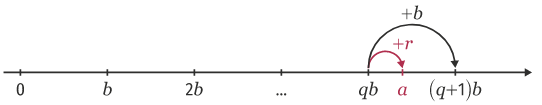
\includegraphics[width = 0.5 \linewidth,valign=c]{div_eucl_axe}

\rems
\begin{enumerate}[a.]
\item La condition $0 \leq r <b$ assure l'unicité du couple $(q ; r)$.
\item Par exemple : Les restes possibles dans la division par 7 sont alors : 0, 1, 2, 3, 4, 5, 6.

\end{enumerate}

\exe Division euclidienne de 412 par 15 : $412=15 \x 27 + 7$. Avec potence : \opidiv{412}{15} 




\prop{On peut étendre la propriété précédente au cas où $a$ est un entier relatif.}

\dem : Admise.

\exe Déterminer le quotient et le reste de la division de $-5000$ par 17.

\begin{minipage}{0.7 \linewidth}
On obtient pour 5000 et 17 : $5000=17 \x 294 +2$.

D'où $-5000 = -17 \x 294 -2$ . Or $-2 \notin \rrbracket 0:17 \rrbracket$ (Point notation)

On en déduit $-5000 = -17 \x 295 + 15$ (on ajoute et enlève 17)

Doù $q=-295 ; r=15$

\end{minipage}
\begin{minipage}{0.25 \linewidth}
\opidiv{5000}{17}
\end{minipage}



\prop{ Soit $b$ un entier naturel tel que $b \geq 2$.

Tout entier $a$ s'écrit sous une, et une seule, des formes $bq,bq+1,bq+2,…,bq+(b-1)$, où $q$ est un entier.}


\dem Soit $a$ un entier.

En effectuant la division euclidienne de $a$ par $b$ non nul, il existe deux entiers naturels $q$ et $r$ tels que $a=bq+r$ avec $0 \leq r <b$.

Par unicité du quotient et du reste $a=bq$ ou $a=bq+1$ ou $a=bq+2$  ... ou $a=bq+(b-1)$.

\medskip

\rema Ainsi, dans la division par 2, le reste est 0 ou 1. Tout entier s'écrit sous la forme $2k$ ou $2k+1$.

On retrouve donc qu'un entier est pair ou impair.

\medskip

\exe Soit $n$ un entier naturel. Posons $A=n(n-2)(n+2)$. Démontrer que $A$ est un multiple de 3.

\textit{Méthode }: D'après le résultat du cours sur la division euclidienne, on sait que tout entier $n$ s'écrit sous une des trois formes suivantes : $n=3k;n=3k+1$ ou $n=3k+2$ avec $k \in \N$.

On raisonne par disjonction de cas en distinguant les trois cas possibles et en démontrant le résultat dans chacun des cas. 


\section{Congruence dans $\Z$}


\defi{Soit $n$ un entier naturel non nul.

Deux entiers $a$ et $b$ sont congrus modulo $n$ lorsque $a-b$ est divisible par $n$.

On note $\modu{a}{b}{n}$
}


\exe Deux nombres de la liste : 1;6;11;16;21;26;31;36 sont congrus modulo 5.

Par exemple pour 21 et 6 : 21-6=15 qui est divisible par 5. On a $\modu{21}{6}{5}$

\prop{Soit $n$ un entier naturel non nul.

Deux entiers $a$ et $b$ sont congrus modulo $n$, si et seulement si, la division euclidienne de $a$ par $n$ a le même reste que la division euclidienne de $b$ par $n$.

}

\dem

$\bullet$ Sens direct : Soient $a$ et $b$ sont congrus modulo $n$.

Par divisions euclidiennes par $n$ on a il existe $(q;r) \in \Z^2$ et $(q',r') \in \Z^2$ tels que $a=nq+r$ et $b=nq'+r'$ avec $0 \leq r <n$ et $0 \leq r' <n$.

On sait qu'il existe $k \in \Z$ tel que $a-b=kn$. ainsi $n(q-q')+r-r'=kn \iff r-r'=n(q-q'-k)$.

Or $-n < r-r' <n$ et $r-r'$ divise $n$ donc $r-r'=0 \iff r=r'$

$\bullet$ Sens indirect : Notons $r$ le même reste que la division euclidienne de $a$ par $n$n et $b$ par $n$.

Par divisions euclidiennes par $n$ on a il existe $q$ et $q'$ tels que $a=nq+r$ et $b=nq'+r$ avec $0 \leq r <n$.

D'où $a-b=n(q-q')=nk$ en posant $k=q-q'$ avec $k \in \Z$. CQFD \medskip


\exe On a vu $\modu{21}{6}{5}$ et $21=4\x5+1;6=1\x5+1$. \medskip

\rems
\begin{enumerate}[$\bullet$]
\item $n$ pair $\iff \modu{n}{0}{2}$ ; $n$ impair $\iff \modu{n}{1}{2}$
\item \raisebox{-3.5mm}{\shadowbox{$n$ est un diviseur de $a$ $\iff \modu{a}{0}{n}$}}
\end{enumerate}

\props { La congruence est une \textbf{relation d'équivalence} c'est-à-dire on a pour tous entiers $a,b,c$ et $n$ :
\begin{enumerate}[$\bullet$]
\item (Réflexivité) $\modu{a}{a}{n}$
\item (Symétrie) $\modu{a}{b}{n} \Rightarrow \modu{b}{a}{n}$
\item (Transitivité) $\modu{a}{b}{n}$ et $\modu{b}{c}{n} \Rightarrow \modu{a}{c}{n}$
\end{enumerate}
}

\dem Découle directement de ce qui précède.

\theo{Soit $n$ un entier naturel ($n \geq 2$), $a$ et $b$ deux entiers relatifs : $\modu{a}{b}{n} \iff \modu{a-b}{0}{n}$.
}


\dem 

$\bullet$ Sens direct : $\modu{a}{b}{n}$ d'où il existe $q,q'$ et $r$ entiers tels que $a=nq+r$ et $b=nq'+r$ avec $0 \leq r <n$.

D'où $a-b=n(q-q') \iff \modu{a-b}{0}{n}$.

$\bullet$ Sens indirect : $\modu{a-b}{0}{n} \iff a-b=kn$ avec $k$ entier.

La division euclidienne de $a$ par $n$n donne $a=nq+r$ avec $0 \leq r <n$ .

D'où par substitution $nq+r-b=kn \iff b = (q-n)+r$. Ainsi $a$ et $b$ ont même reste dans la division euclidienne par $n$.

\medskip

\props { \textbf{Compatibilité avec certaines opérations} :

Soient $n$ un entier naturel non nul et $a,b,a',b'$ des nombres relatifs tels que $\modu{a}{b}{n}$ et $\modu{a'}{b'}{n}$ alors on a :

\begin{multicols}{2}
\begin{enumerate}[$\bullet$]
\item Addition : $\modu{a+a'}{b+b'}{n}$
\item Soustraction : $\modu{a-a'}{b-b'}{n}$
\item Produit : $\modu{a \x a'}{b \x b'}{n}$
\item Puissance : $\modu{a^p}{b^p}{n}$
\end{enumerate}
\end{multicols}
}

\dem 

$\bullet$ Addition : $\left\lbrace \begin{array}{l} \modu{a}{b}{n} \\ \modu{a'}{b'}{n} \end{array} \right.
\iff \left\lbrace \begin{array}{l} \modu{a-b}{0}{n} \\ \modu{a'-b'}{0}{n} \end{array} \right. \iff 
\left\lbrace \begin{array}{l} a-b=kn \\ a'-b'=k'n \end{array} \right.$ avec $k,k'$ entiers.

$(a-b)+(a'-b')=kn+k'n \iff (a+a')-(b-b')=(k+k')n \iff \modu{a+a'}{b+b'}{n}$.

$\bullet$ Multiplication : $\left\lbrace \begin{array}{l} \modu{a}{b}{n} \\ \modu{a'}{b'}{n} \end{array} \right.
\iff \left\lbrace \begin{array}{l} a=b+kn \\ a'=b'+k'n \end{array} \right.$

$aa'=bb'+nK$ avec $K=bk'+b'k +kk'n \in \Z$ i.e. $\modu{aa'}{bb'}{n}$

$\bullet$ Puissance : Par récurrence.

\textbf{Initialisation} : trivial pour $p=0$ ou $p=1$.

\textbf{Hérédité }: Supposons qu'il existe un entier $k$ tel que la propriété $P(k) : \modu{a^p}{b^p}{n}$  soit vraie.

Alors $a^{k+1} \equiv a^k \x a \equiv b^k \x b \equiv b^{k+1} ~[n]$.

\textbf{Conclusion} : La propriété est vraie pour $p=0$ et héréditaire à partir de ce rang. D'après le principe de récurrence, elle est vraie pour tout entier naturel $p$.



\exes
\begin{enumerate}[a.]
\item On a $\modu{7}{4}{3}$ et $\modu{11}{20}{3}$ d'où 

$\modu{7+11}{4+20}{3} \iff \modu{18}{24}{3}$

$\modu{7 \x 11}{4 \x 20}{3} \iff \modu{77}{80}{3} \iff \modu{77}{2}{3}$

\item $\modu{22}{1}{7}$ d'où $\modu{22^{50}}{1}{7}$

$\modu{59}{3}{7}$ d'où $\modu{59^3}{2^3}{7} \iff \modu{59^3}{1}{7}$.

\end{enumerate}


\exe Déterminer le reste de la division de $2^{437}$ par 7.

Méthode :

On cherche une puissance de 2 congrue à 1 modulo 7. on trouve $\modu{2^3}{1}{7}$.

On décompose 497 avec la division euclidienne par 3 : $497=3 \x 145 + 2$.

Ainsi $2^{437} \equiv 2^{3 \x 145 +2} \equiv \left(2^3 \right)^{145} \x 2^2 \equiv 1^{145} \x 4 \equiv 4 [7]$

\medskip

\exe Résoudre une équation avec des congruences
\begin{enumerate}[a.]
\item Déterminer les entiers $x$ tels que $\modu{6+x}{5}{3}$
\item Déterminer les entiers $x$ tels que $\modu{3x}{5}{4}$

\end{enumerate}


a. $\modu{6+x}{5}{3} \iff \modu{x}{-1}{3} \iff \modu{x}{2}{3}$.

Les entiers $x$ solutions sont les entiers de la forme $2+3k$ avec $k \in \Z$.

b. $\modu{3x}{5}{4} \iff \modu{3x}{1}{4}$.

$x$ est nécessairement congru soit à 0,1,2 ou 3 modulo 4.

Par disjonction de cas on obtient : \begin{tabular}{|c|c|c|c|c|}
\hline 
$x$ modulo 4 & 0 & 1 & 2 & 3 \\ 
\hline 
$3x$ modulo 4 & 0 & 3 & 2 & 1 \\ 
\hline 
\end{tabular} 

Seul $\modu{x}{3}{4}$ convient ainsi les entiers $x$ solutions sont les entiers de la forme $3+4k$ avec $k \in \Z$.

\end{document}	







